\documentclass[tikz,border=10pt]{standalone}
\usepackage{tikz}
\begin{document}
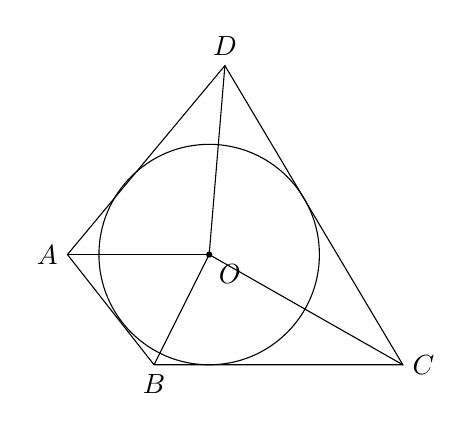
\begin{tikzpicture}[scale=2]
  % Define the vertices of the quadrilateral
  \coordinate (A) at (0,0.1);
  \coordinate (B) at (0.55,-0.6);
  \coordinate (C) at (2.13,-0.6);
  \coordinate (D) at (1,1.3);
  
  % Define the center O
  \coordinate (O) at (0.9,0.1);
  
  % Draw the quadrilateral
  \draw (A) -- (B) -- (C) -- (D) -- cycle;
  \draw (A) -- (O);
  \draw (B) -- (O);
  \draw (C) -- (O);
  \draw (D) -- (O);
  
  % Draw the inscribed circle
  \draw (O) circle (0.7);

  % Mark the center O
  \fill (O) circle (0.02);
  
  % Label the vertices
  \node[left] at (A) {$A$};
  \node[below] at (B) {$B$};
  \node[right] at (C) {$C$};
  \node[above] at (D) {$D$};
  \node[below right] at (O) {$O$};
  
\end{tikzpicture}
\end{document}